\documentclass{article}

\usepackage{fancyhdr}
\usepackage{extramarks}
\usepackage{amsmath}
\usepackage{amsthm}
\usepackage{amsfonts}
\usepackage{tikz}
\usepackage[plain]{algorithm}
\usepackage{algpseudocode}

\usetikzlibrary{automata,positioning}

%
% Basic Document Settings
%

\topmargin=-0.45in
\evensidemargin=0in
\oddsidemargin=0in
\textwidth=6.5in
\textheight=9.0in
\headsep=0.25in

\linespread{1.1}

\pagestyle{fancy}
\lhead{\hmwkAuthorName}
\chead{\hmwkClass\ (\hmwkClassInstructor): \hmwkTitle}
\rhead{\firstxmark}
\lfoot{\lastxmark}
\cfoot{\thepage}
\usetikzlibrary{trees}

\renewcommand\headrulewidth{0.4pt}
\renewcommand\footrulewidth{0.4pt}

\setlength\parindent{0pt}

%
% Create Problem Sections
%

\newcommand{\enterProblemHeader}[1]{
	\nobreak\extramarks{}{Problem \arabic{#1} continued on next page\ldots}\nobreak{}
	\nobreak\extramarks{Problem \arabic{#1} (continued)}{Problem \arabic{#1} continued on next page\ldots}\nobreak{}
}

\newcommand{\exitProblemHeader}[1]{
	\nobreak\extramarks{Problem \arabic{#1} (continued)}{Problem \arabic{#1} continued on next page\ldots}\nobreak{}
	\stepcounter{#1}
	\nobreak\extramarks{Problem \arabic{#1}}{}\nobreak{}
}

\setcounter{secnumdepth}{0}
\newcounter{partCounter}
\newcounter{homeworkProblemCounter}
\setcounter{homeworkProblemCounter}{1}
\nobreak\extramarks{Problem \arabic{homeworkProblemCounter}}{}\nobreak{}

%
% Homework Problem Environment
%
% This environment takes an optional argument. When given, it will adjust the
% problem counter. This is useful for when the problems given for your
% assignment aren't sequential. See the last 3 problems of this template for an
% example.
%
\newenvironment{homeworkProblem}[1][-1]{
	\ifnum#1>0
		\setcounter{homeworkProblemCounter}{#1}
	\fi
	\section{Problem \arabic{homeworkProblemCounter}}
	\setcounter{partCounter}{1}
	\enterProblemHeader{homeworkProblemCounter}
}{
	\exitProblemHeader{homeworkProblemCounter}
}

%
% Homework Details
%   - Title
%   - Due date
%   - Class
%   - Section/Time
%   - Instructor
%   - Author
%

\newcommand{\hmwkTitle}{Problem Set\ \#8}
\newcommand{\hmwkDueDate}{Jun 16, 2025}
\newcommand{\hmwkClass}{ECON 121}
\newcommand{\hmwkClassInstructor}{Dr. Jasmine N Fuller}
\newcommand{\hmwkAuthorName}{\textbf{Alejandro Ouslan}}

%
% Title Page
%

\title{
	\vspace{2in}
	\textmd{\textbf{\hmwkClass:\ \hmwkTitle}}\\
	\normalsize\vspace{0.1in}\small{Due\ on\ \hmwkDueDate}\\
	\vspace{0.1in}\large{\textit{\hmwkClassInstructor}}
	\vspace{3in}
}

\author{\hmwkAuthorName}
\date{}

\renewcommand{\part}[1]{\textbf{\large Part \Alph{partCounter}}\stepcounter{partCounter}\\}

%
% Various Helper Commands
%

% Useful for algorithms
\newcommand{\alg}[1]{\textsc{\bfseries \footnotesize #1}}

% For derivatives
\newcommand{\deriv}[1]{\frac{\mathrm{d}}{\mathrm{d}x} (#1)}

% For partial derivatives
\newcommand{\pderiv}[2]{\frac{\partial}{\partial #1} (#2)}

% Integral dx
\newcommand{\dx}{\mathrm{d}x}

% Alias for the Solution section header
\newcommand{\solution}{\textbf{\large Solution}}

% Probability commands: Expectation, Variance, Covariance, Bias
\newcommand{\E}{\mathrm{E}}
\newcommand{\Var}{\mathrm{Var}}
\newcommand{\Cov}{\mathrm{Cov}}
\newcommand{\Bias}{\mathrm{Bias}}

\begin{document}

\maketitle

\pagebreak

% Homework problem 1
\begin{homeworkProblem}
	You have \$100 to invest and are wondering where to put it. You are considering whether to buy your
	favorite stock (B) or put it in your couch (C), either decision occurring today. You know the stock price
	today, conveniently enough \$100 per share, but you don’t know the stock price tomorrow. For simplicity,
	it could either be double (\$200) or nothing (\$0), with the probability of double being $p$, and the
	probability of nothing being $1 - p$. If you invest in your couch you get your \$100 back tomorrow. Your
	discount factor is $\delta$, and you are risk neutral (i.e. your payoffs only depend on time discounting and
	money.)

	\begin{enumerate}
		\item Draw the complete game tree, with nature and player 1.

		      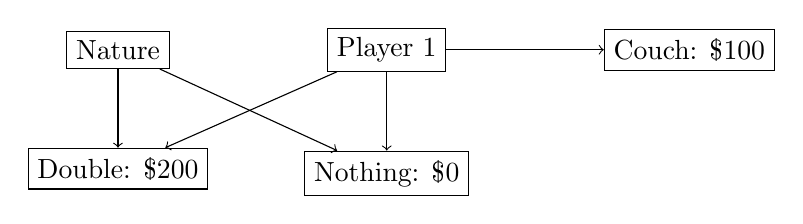
\begin{tikzpicture}
			      \node[draw] (nature) {Nature};
			      \node[draw, right=2cm of nature] (player) {Player 1};
			      \node[draw, below=1cm of nature] (double) {Double: \$200};
			      \node[draw, below=1cm of player] (nothing) {Nothing: \$0};
			      \node[draw, right=2cm of player] (couch) {Couch: \$100};

			      \draw[->] (nature) -- (double);
			      \draw[->] (nature) -- (nothing);
			      \draw[->] (player) -- (couch);
			      \draw[->] (player) -- (double);
			      \draw[->] (player) -- (nothing);
		      \end{tikzpicture}

		\item At what level of $p$ should you buy you favorite stock?

		      \[
			      E[\text{Payoff from stock}] = p \cdot \frac{200}{1+\delta} + (1-p) \cdot \frac{0}{1+\delta}
		      \]
		      \[
			      E[\text{Payoff from couch}] = \frac{100}{1+\delta}
		      \]

		      \[
			      p \cdot \frac{200}{1+\delta} > \frac{100}{1+\delta}
		      \]
		      \[
			      p > \frac{1}{2}
		      \]

		      Thus, you should buy the stock if \( p > \frac{1}{2} \).

		\item Why doesn't $\delta$ affect part (b)?

		      $\delta$ cancels out in the inequality.
		\item Suppose $p$ is greater than you answer in part (b). Martha Stewart knows what the stok price is
		      going to be tomorrow, and offers to sell this information to you. You trust that she knows and is
		      being honest because her written offer is finely hand-crafted using everyday houshold items.
		      Assuming you only concern is making money and discounting for time (instead of moral quams),
		      or going to prison), how much would you be willing to pay for this information?


		      \[
			      \text{Expected Payoff with Information} = p \cdot \frac{200}{1+\delta} + (1-p) \cdot \frac{100}{1+\delta}
		      \]

		      \[
			      \text{Willingness to Pay} = \left( p \cdot \frac{200}{1+\delta} + (1-p) \cdot \frac{100}{1+\delta} \right) - \left( p \cdot \frac{200}{1+\delta} + (1-p) \cdot \frac{0}{1+\delta} \right)
		      \]
		      \[
			      \text{Willingness to Pay} = (1 - p) \cdot \frac{100}{1+\delta}
		      \]

		      Thus, the maximum amount you would be willing to pay for the information is:
		      \[
			      (1 - p) \cdot \frac{100}{1+\delta}
		      \]


	\end{enumerate}
\end{homeworkProblem}

% Homework problem 2 
\begin{homeworkProblem}
	There was an old game show called “Let’s Make a Deal” hosted by Monty Hall. In it was a game where a
	prize was hidden behind one of three doors, and behind the other two doors were goats. The contestant
	initially chose a door; then Monty Hall would open one of the doors the contestant did not pick to reveal a
	goat. Then the contestant had the option to stay with the door he chose or switch to the other un-opened
	door.

	Suppose you are playing this game, the “prize” is worth \$10,000, and a goat is worth nothing. Since it’s
	random anyway, you already chose door A (the decision is “sunk” and is not part of the game directly).
	The game starts as nature randomly determines where the prize is (1/3 chance for any of the three doors);
	then Monty Hall selects one of doors B or C that has a goat (also a move by nature); then you choose to
	Stay at door A or to Switch to the unopened door. Finally, the outcome is resolved – either you find a goat
	or the prize behind the door you finally selected.

	If both B and C have a goat, Monty flips a coin (50/50 chance) to determine which one to open. If either
	B or C have the car, there is only one available door Monty can open, so he opens that one.

	Now, we draw the complete game tree; I detail it in several steps to try and help you

	\begin{enumerate}
		\item Draw the first mover, Nature, picking which door has the prize, A,B,or C. Make sure to include
		      probabilities!
		      \[
			      P(\text{Prize behind A}) = \frac{1}{3}, \quad P(\text{Prize behind B}) = \frac{1}{3}, \quad P(\text{Prize behind C}) = \frac{1}{3}
		      \]
		\item Draw the second mover, Nature (again!). picking which door to open - B or C. If it's a
		      degenerate lottery, you don't have to actully draw a new branch of the tree. But when it isn't a
		      degenerate lottery, you actually have to draw out the branches of the decision tree and think about
		      what is happening.


		      In this case, Monty can open either B or C with equal probability because both doors have goats.

		      \[
			      P(\text{Monty opens B} | \text{Prize behind A}) = \frac{1}{2}, \quad P(\text{Monty opens C} | \text{Prize behind A}) = \frac{1}{2}
		      \]


		      Monty must open door C in this case because it’s the only remaining door with a goat.

		      \[
			      P(\text{Monty opens C} | \text{Prize behind B}) = 1
		      \]


		      Monty must open door B in this case because it’s the only remaining door with a goat.

		      \[
			      P(\text{Monty opens B} | \text{Prize behind C}) = 1
		      \]

		\item Draw the third and final mover, the player (you), picking either to Stay at door A or Switch to the only
		      other door available.
		      The player now has the option to either Stay with door A or Switch to the other door. The outcomes are dependent on the prize's location and Monty’s choice of which door to open.


		      - If the player stays at A, they win the prize (\$10,000).
		      - If the player switches, they get a goat (\$0).

		      \[
			      P(\text{Win by staying at A} | \text{Prize behind A}) = 1, \quad P(\text{Win by switching}) = 0
		      \]


		      - If the player stays at A, they get a goat (\$0).
		      - If the player switches to C, they get a goat (\$0).

		      \[
			      P(\text{Win by staying at A} | \text{Prize behind B}) = 0, \quad P(\text{Win by switching}) = 0
		      \]


		      - If the player stays at A, they get a goat (\$0).
		      - If the player switches to B, they get a goat (\$0).

		      \[
			      P(\text{Win by staying at A} | \text{Prize behind C}) = 0, \quad P(\text{Win by switching}) = 0
		      \]

		      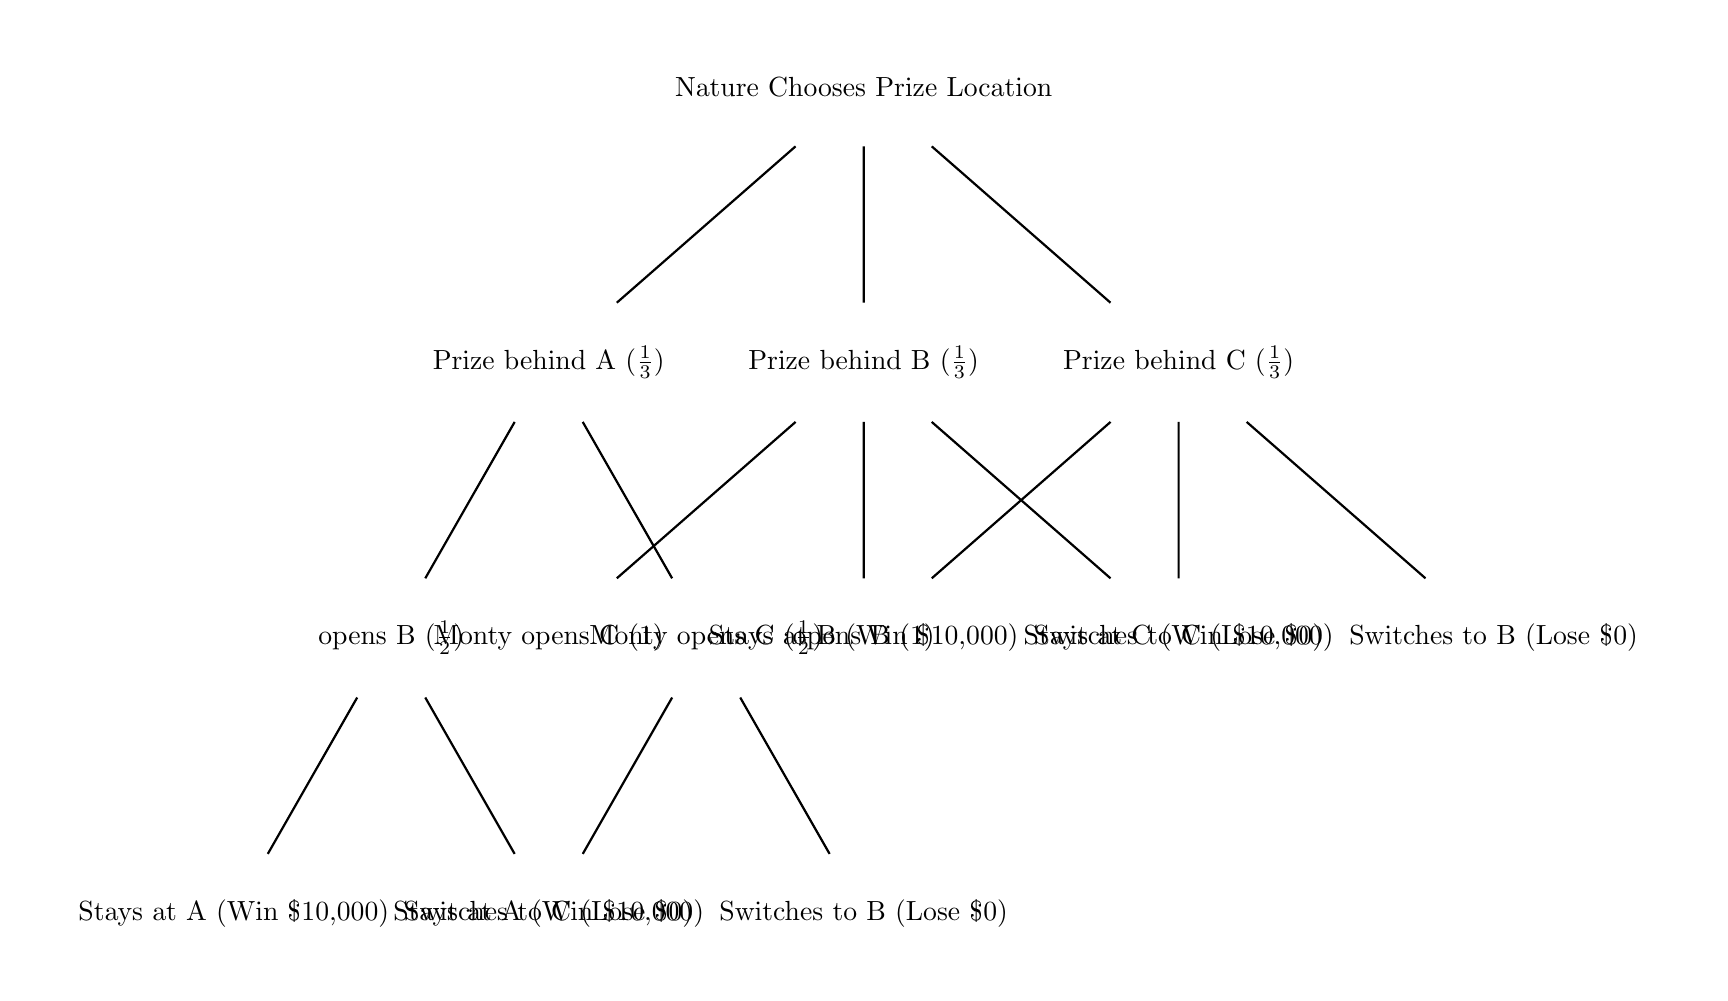
\begin{tikzpicture}[edge from parent/.style={draw,thick,black,-},
				      grow=down,
				      level distance=3.5cm,
				      sibling distance=4cm,
				      every node/.style={text width=5cm, align=center, minimum height=1.5cm}]
			      % Nature chooses the prize location
			      \node {Nature Chooses Prize Location}
			      child {node {Prize behind A (\(\frac{1}{3}\))}
					      child {node {opens B (\(\frac{1}{2}\))}
							      child {node {Stays at A (Win \$10,000)}}
							      child {node { Switches to C (Lose \$0)}}}
					      child {node {Monty opens C (\(\frac{1}{2}\))}
							      child {node {Stays at A (Win \$10,000)}}
							      child {node {Switches to B (Lose \$0)}}}
				      }
			      child {node {Prize behind B (\(\frac{1}{3}\))}
					      child {node {Monty opens C (1)}}
					      child {node {Stays at B (Win \$10,000)}}
					      child {node {Switches to C (Lose \$0)}}}
			      child {node {Prize behind C (\(\frac{1}{3}\))}
					      child {node {opens B (1)}}
					      child {node {Stays at C (Win \$10,000)}}
					      child {node {Switches to B (Lose \$0)}}};
		      \end{tikzpicture}

		\item Finally, list the payoffs at each terminal node. It's either \$10,000 if the player's decision led to the
		      prize, or \$0if it didn't

		      \begin{itemize}
			      \item If the player stays at A and the prize is behind A, the payoff is \$10,000.
			      \item If the player switches to C and the prize is behind A, the payoff is \$0.
			      \item If the player stays at A and the prize is behind B, the payoff is \$0.
			      \item If the player switches to C and the prize is behind B, the payoff is \$0.
			      \item If the player stays at A and the prize is behind C, the payoff is \$0.
			      \item If the player switches to B and the prize is behind C, the payoff is \$0.
		      \end{itemize}


		\item Using that big, wonderful game tree, calculate the probility you get the prize (\$10,000) for each
		      combination: Door B has a goat and you Stay (pick A), Door B has a goat and you Switch (pick C),
		      Door C has a goat and you Stay (pick A), Door B has a goat and you Switch (pick B).

		      \begin{itemize}
			      \item \textbf{Door B has a goat, and you Stay at A:}
			            The probability is the chance that the prize is behind A and Monty opens either B or C. This is
			            \[
				            \frac{1}{3} \times \frac{1}{2} = \frac{1}{6}
			            \]
			      \item \textbf{Door B has a goat, and you Switch to C:}
			            The probability is the chance that the prize is behind A, Monty opens B, and the player switches. This is
			            \[
				            \frac{1}{3} \times \frac{1}{2} = \frac{1}{6}
			            \]
			      \item \textbf{Door C has a goat, and you Stay at A:}
			            The probability is the chance that the prize is behind A and Monty opens C. This is
			            \[
				            \frac{1}{3} \times \frac{1}{2} = \frac{1}{6}
			            \]
			      \item \textbf{Door B has a goat, and you Switch to B:}
			            The probability is the chance that the prize is behind B and Monty opens C. This is
			            \[
				            \frac{1}{3} \times 1 = \frac{1}{3}
			            \]
		      \end{itemize}

		\item What should you do?

		      The best strategy is to \textbf{Switch}, as it maximizes the chance of winning the prize.

	\end{enumerate}


\end{homeworkProblem}

\end{document}
